\chapter{Active Debugging}
\label{sec:guided-approach}


\begin{figure}[!ht]
	\centering
	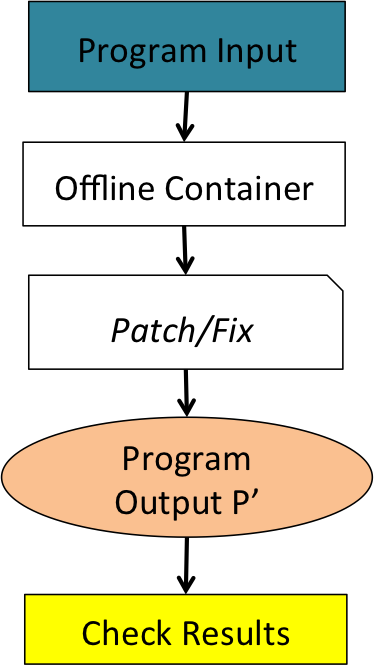
\includegraphics[width=0.25\textwidth]{guided/figs/offline.png}
	\label{fig:offlineDebugging}
	\caption{Debugging strategies for offline debugging}
\end{figure}


\section{Overview}

In this section, we introduce \activedebugging whereby developers can apply a patch/fix or apply a test in the \debugcontainer.
\activedebugging ensures that any modifications in the \debugcontainer does not lead to a state change in the \productioncontainer.
This will enable the debugger to fix/patch or run test-cases in the debug-container while ensuring forward progress and in sync with production. 
We are inspired from existing perpetual invivo testing frameworks like INVITE~\cite{invivo}(which also provides partial test-isolation), in the production environment.
We currently restrict \active debugging to patches/and test-cases only bring about local changes, and not global changes in the application.

\section{Description}

In Figure~\ref{fig:offlineDebugging}, we show the traditional mechanism of testing or validating patch/fixes in an application. 
In offline environments, developers apply patches and run the relevant inputs to verify that the patch works correctly. 
This is an interactive process, which allows one to verify the result and corrections before applying it to the production system.
Several cycles of this process is required, which may be followed by staged testing to ensure correctness before applying the update to the production.


\emph{Active Debugging} (see figure~\ref{fig:active-debugging}) allows debuggers to apply fixes, modify binaries and apply hotpatches to applications. 
The main idea is to do a fork/exec, or parallel execution of an unmodified application.
The unmodified binary continues execution without any change in the input.
The debug-container should ideally mimic the behavior of the production, so as to allow for forward progress in the application as the debug-container will receive the same input as production.
The target process will be forked at the call of the testing function, the forked process can then be tested, the input can be transformed, or alternatively the same input can be used to validate any test-condition. 
At the end of the execution the test-process output can be checked and killed. 
The advantage of this technique is that any tests/fixes can be validated in the run-time environment itself.
This reduces the time to fix and resolve the error. 
The tests and fixes should have a local impact and should not be allowed to continue 


\begin{figure}[!ht]
	\centering
	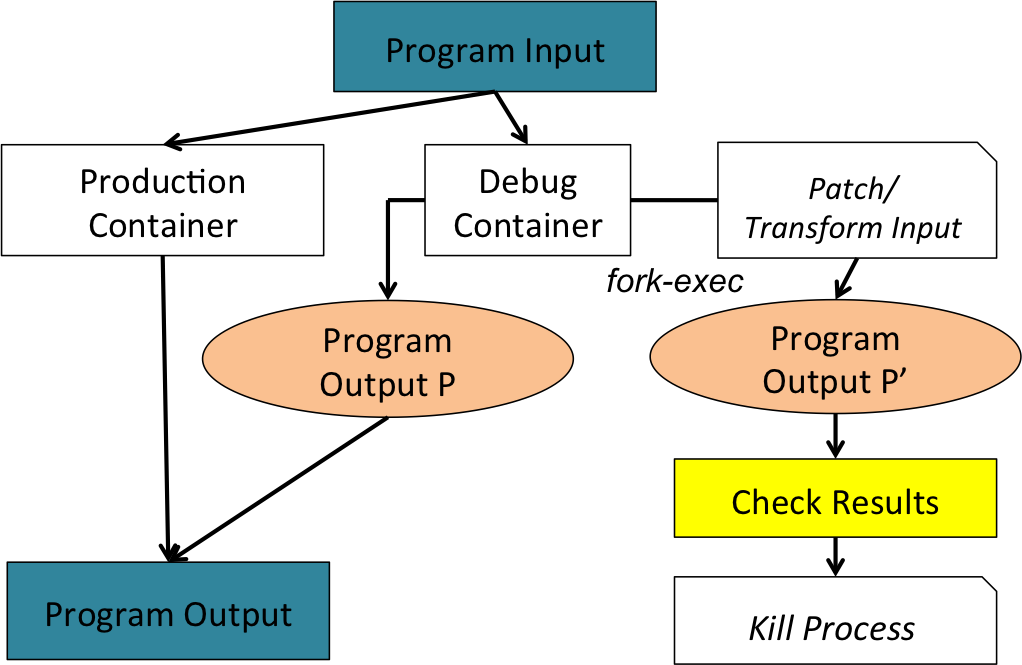
\includegraphics[width=0.75\textwidth]{guided/figs/active-debugging.png}
	\label{fig:active-debugging}
	\caption{Debugging Strategies for Active Debugging}
\end{figure}

For Java programs, since there is no “fork”, we can utilize a JNI call to a simple native C program which executes the fork. 
Performing a fork creates a copy-on-write version of the original process, so that the process running the unit test has its own writable memory area and cannot affect the in-process memory of the original. 
Once the test is invoked, the application can continue its normal execution, while the unit test runs in the other process. 
Note that the application and the unit test run in parallel in two processes; the test does not block normal operation of the application after the fork is performed.

The fork-exec design of test-isolation ensures that the ``in-process'' memory of the process execution is effectively isolated. 
The production/debug containers are completely isolated hence the test does not impact the production in any way. 
To ensure further isolation, we can allow the test fork to only call wrapper libraries which allow write operations in a cloned cow filesystem.
This can be done using a COW supported file-system with cloning functionality which are supported in ZFS and BTRFS.
For instance BTRFS provides a clone operation that atomically creates a copy-on-write snapshot of a file. By cloning the file system does not create a new link pointing to an existing inode; instead it creates a new inode that initially shares the same disk blocks with the original file. As a result cloning works only within the boundaries of the same BTRFS file system, and modifications to any of the cloned files are not visible to the original file and vice versa. 
This will of-course mean that we will constrain the debug/production environment to the File System of our choice.
All test-cases in the debug-container share the test file system.
